%%%%%%%%%%%%%%%
%
% $Autor: Wings $
% $Datum: 2020-01-29 07:55:27Z $
% $Pfad: General/OLED.tex
% $Version: 1785 $
%
%
%%%%%%%%%%%%%%%

\chapter{OLED-Display}


\Mynote{Wo sind die Programmdateien?\\
Version der Bibliothek?\\
Welche Möglichkeiten?\\
Was ist OLED?\\
Funktionsbeschreibungen?\\
Grafiken?
\ldots}


\section{OLED}

Im Folgenden wird das Display  DEBO OLED2 0.96 beschrieben. Dieses kleine Display mit einem schwarzen Hintergrund und blauer Anzeigefarbe lässt sich mit I\textsuperscript{2}C ansteuern. Die hohe Auflösung bietet ein scharfes Bild.\cite{Simac:2019}

\bigskip

Technische Daten:

\begin{itemize}
  \item Auflösung: 128 $\times$ 64 Pixel
  \item Hintergrundfarbe: Schwarz
  \item Anzeigefarbe: blau
  \item Maße: 27 mm $\times$  27 mm $\times$ 11 mm
  \item Anschluss: 4-polig Anschluss
  \item Interface: I\textsuperscript{2}C
  \item SSD-Controller: SSD1306
  \item Spannungsversorgung: 3,3 - 5 V
\end{itemize}


\Mynote{Schaltbild, Anschlüsse? Stromverbrauch? Lebensdaur?\ldots}
\section{Anschluss}

In der Abbildung \ref{OLEDCurcuit} ist einer Schaltplan  zu sehen, in dem das Display verwendet wird. Die Masse des OLED-Displays ist in der Farbe schwarz gekennzeichnet und ist  über das Arduino Shield an den Masse Port des Arduino verbunden. Die  Spannungsversorgung mit 3,3V für das OLED-Display ist in rot gekennzeichnet. Die beiden Pins für die Datenübertragung und für das OLED-Display gehen in die vorgesehen SDA und SCL Pins am Arduino.
\Mynote{Farbe und Nummer?}

\begin{figure}
    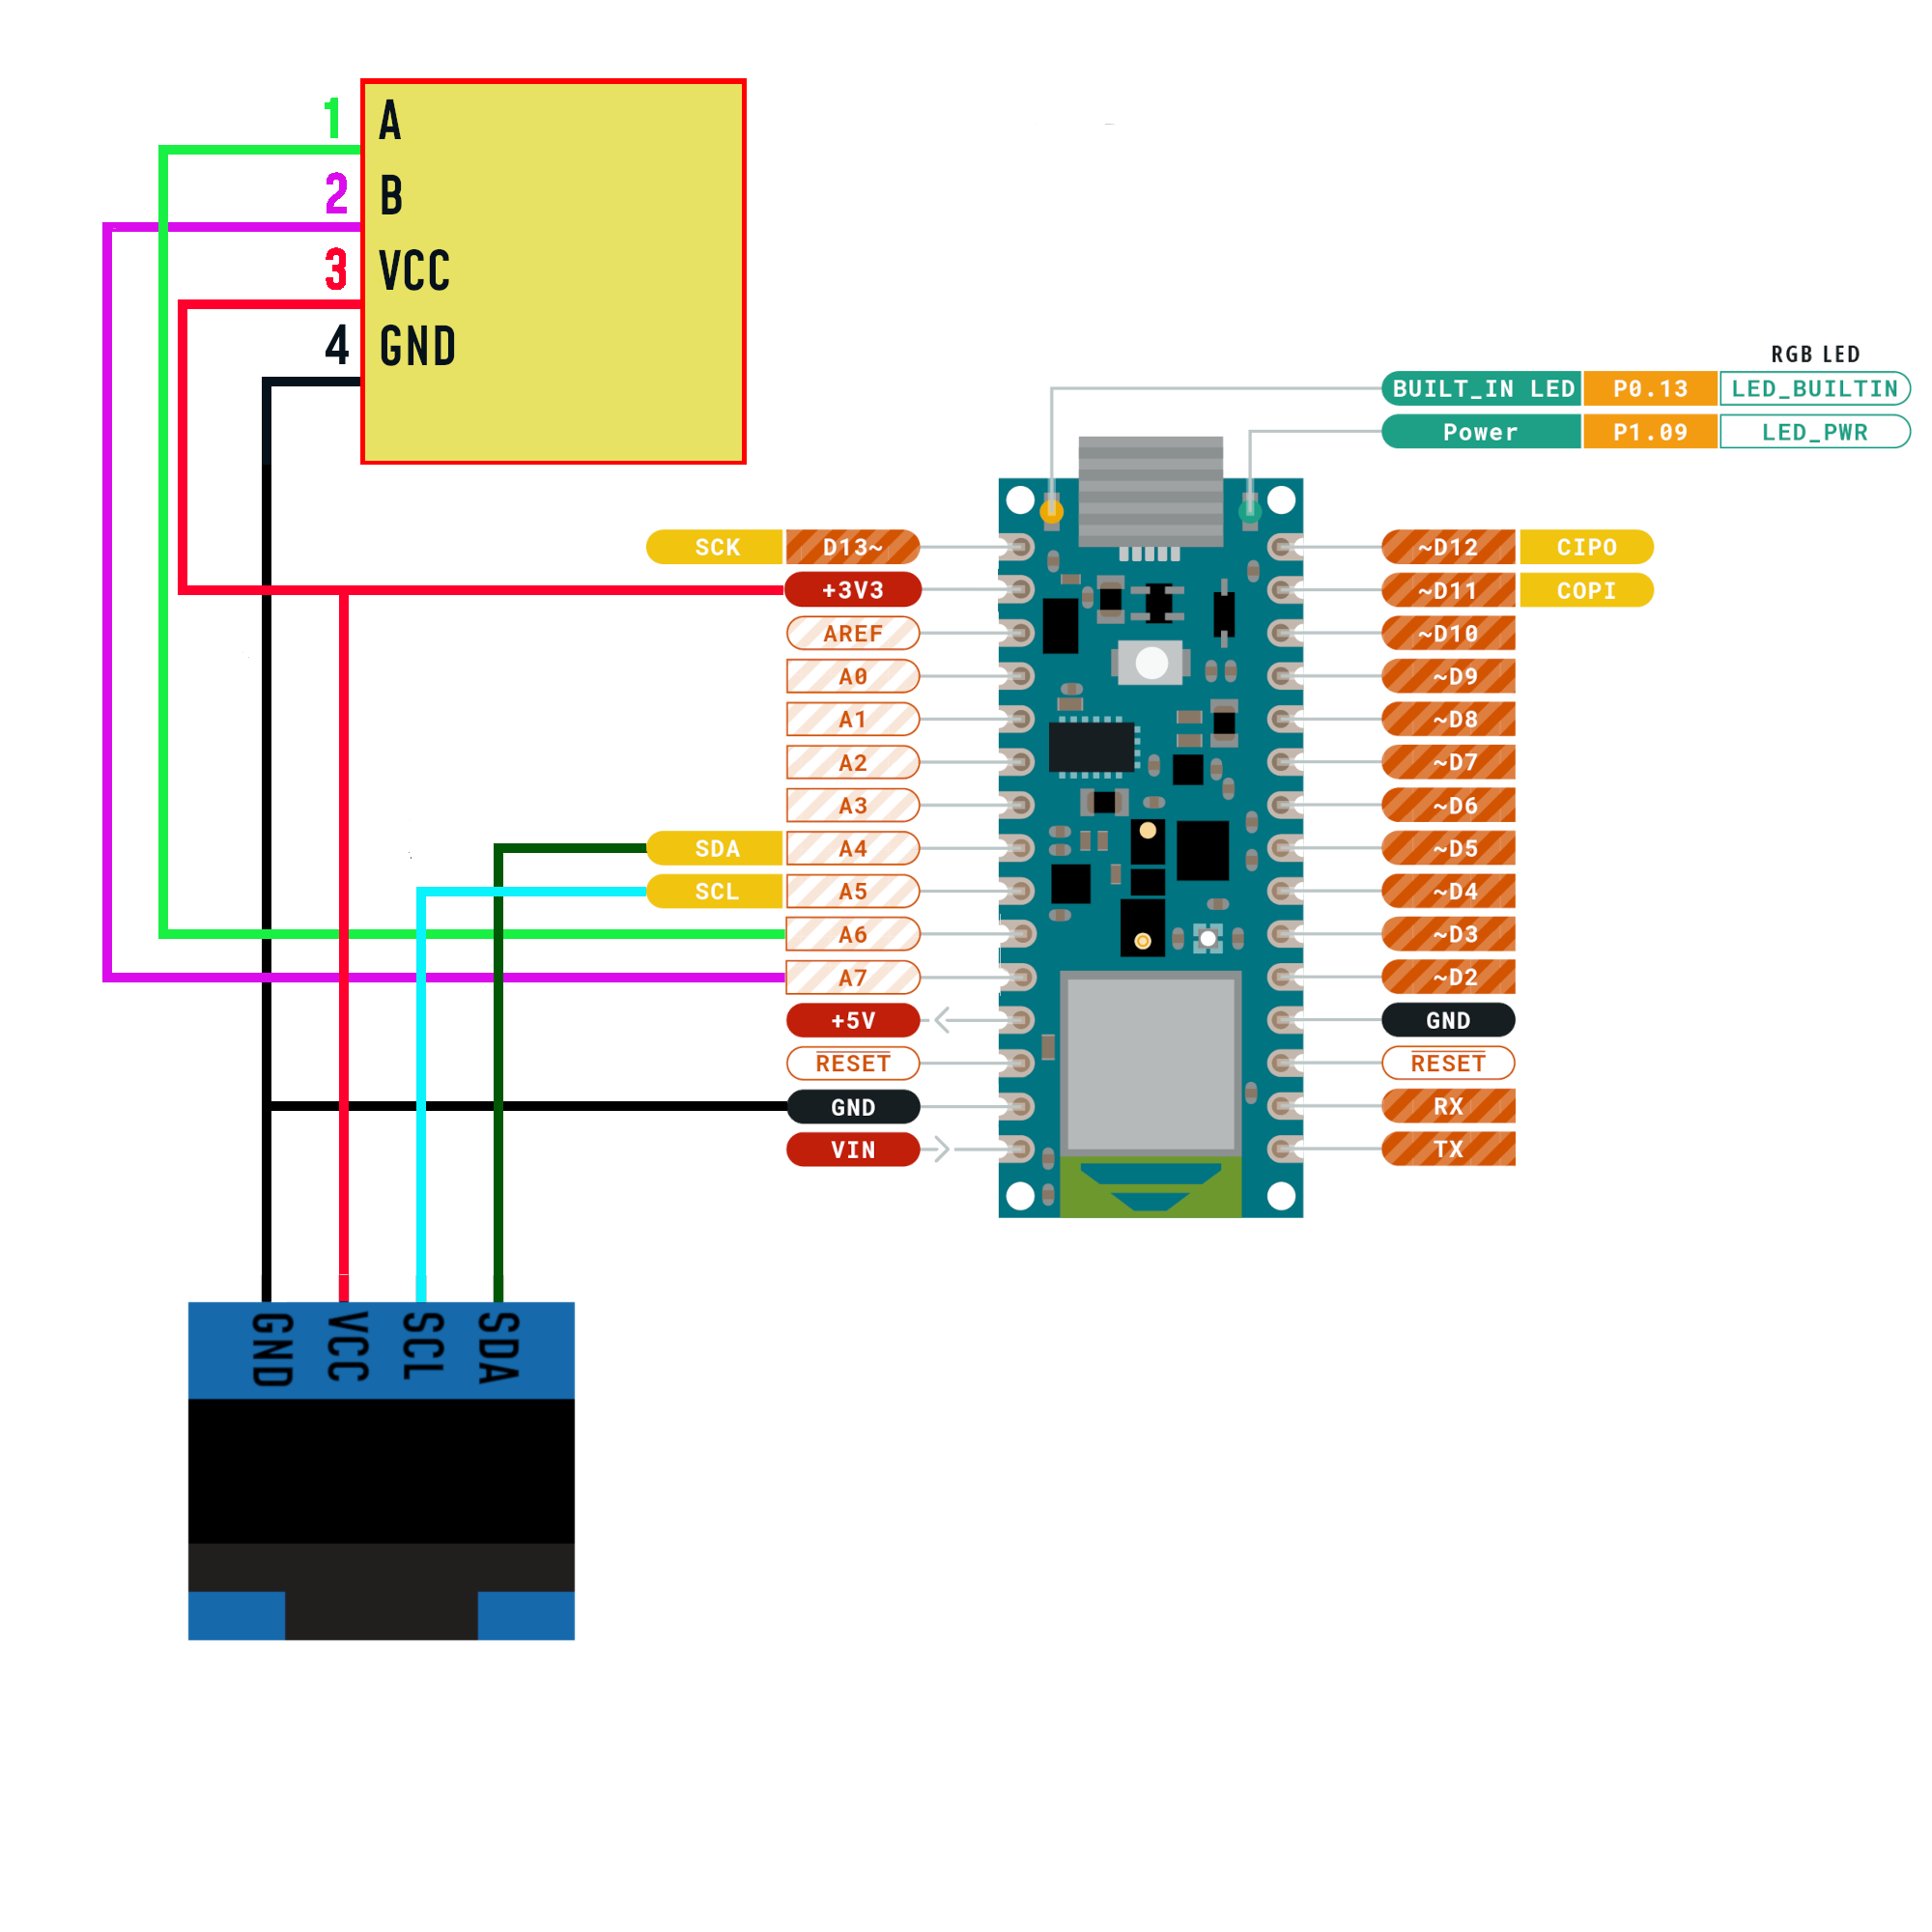
\includegraphics[width=12cm]{OLED/OLEDCircuit2}
    \caption{Gesamter Schaltplan}\label{OLEDCurcuit}
\end{figure}

\Mynote{Nur Display darstellen}

\section{Programmierung}
\subsection{\textcolor{FileColor}{Wire.h}}

Die \textcolor{FileColor}{Wire.h} Bibliothek gehört nicht zu den spezielleren Bibliotheken. Trotzdem spielt sie eine wichtige funktionale Rolle, da durch sie die Verbindung zwischen dem Arduino und dem OLED-Display ermöglicht wird. \textcolor{FileColor}{Wire.h} kommt immer dann zum Einsatz, wenn eine Kommunikation über I2C erfolgen soll. Die Datenübertragung mittels I2C geschieht über die zwei Anschlüsse SDA und SCL. SDA ist eine serielle Datenübertragungsleitung und SCL sendet die erforderlichen Taktimpulse. Diese beiden Leitungen bilden in Kombination mit der Spannungsversorgung, 3V3 und GND, alle benötigten Anschlüsse, um das Display mit dem Arduino zu verbinden.   


\subsection{OLED-Display}

Das OLED-Display benötigt, wie zuvor erwähnt, die  Bibliothek SSD1306Ascii. In ihr sind jegliche Funktionen implementiert, um das Display individuell einzurichten. Mithilfe der ebenfalls herunterzuladenden Beispiele, ermöglicht man dem Anwender so einen schnellen Funktionstest. So kann beispielsweise überprüft werden, ob das Display korrekt angeschlossen ist und ob die Ausgabe funktioniert.

\begin{figure}[H]
    \centering
    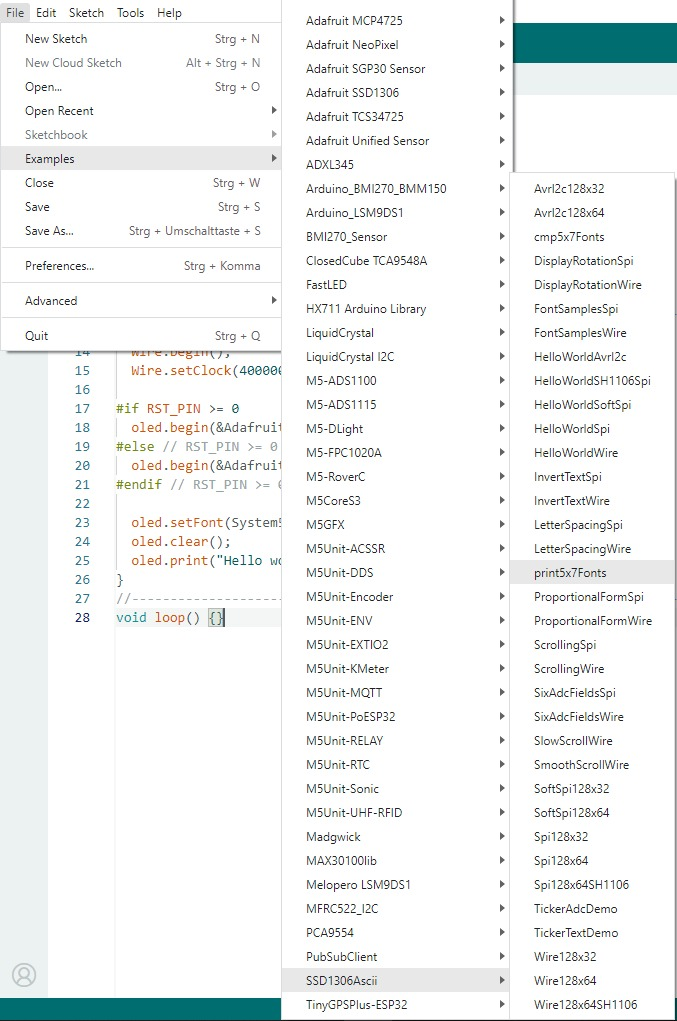
\includegraphics[width=0.7\textwidth]{OLED/OLEDBibliothek}
    \caption{Beispiele in der OLED Bibliothek}
\end{figure}

\subsection{Testen des OLED-Displays}

Auf dem OLED-Display wurde das Beispiel \FILE{HelloWorldWire} geladen, um die richtige Ausgabe des Displays zu gewährleisten. Wie in Abbildung 4.4 zu sehen ist, zeigt das Display die erwartete Ausgabe an.

\begin{figure}
    \centering
    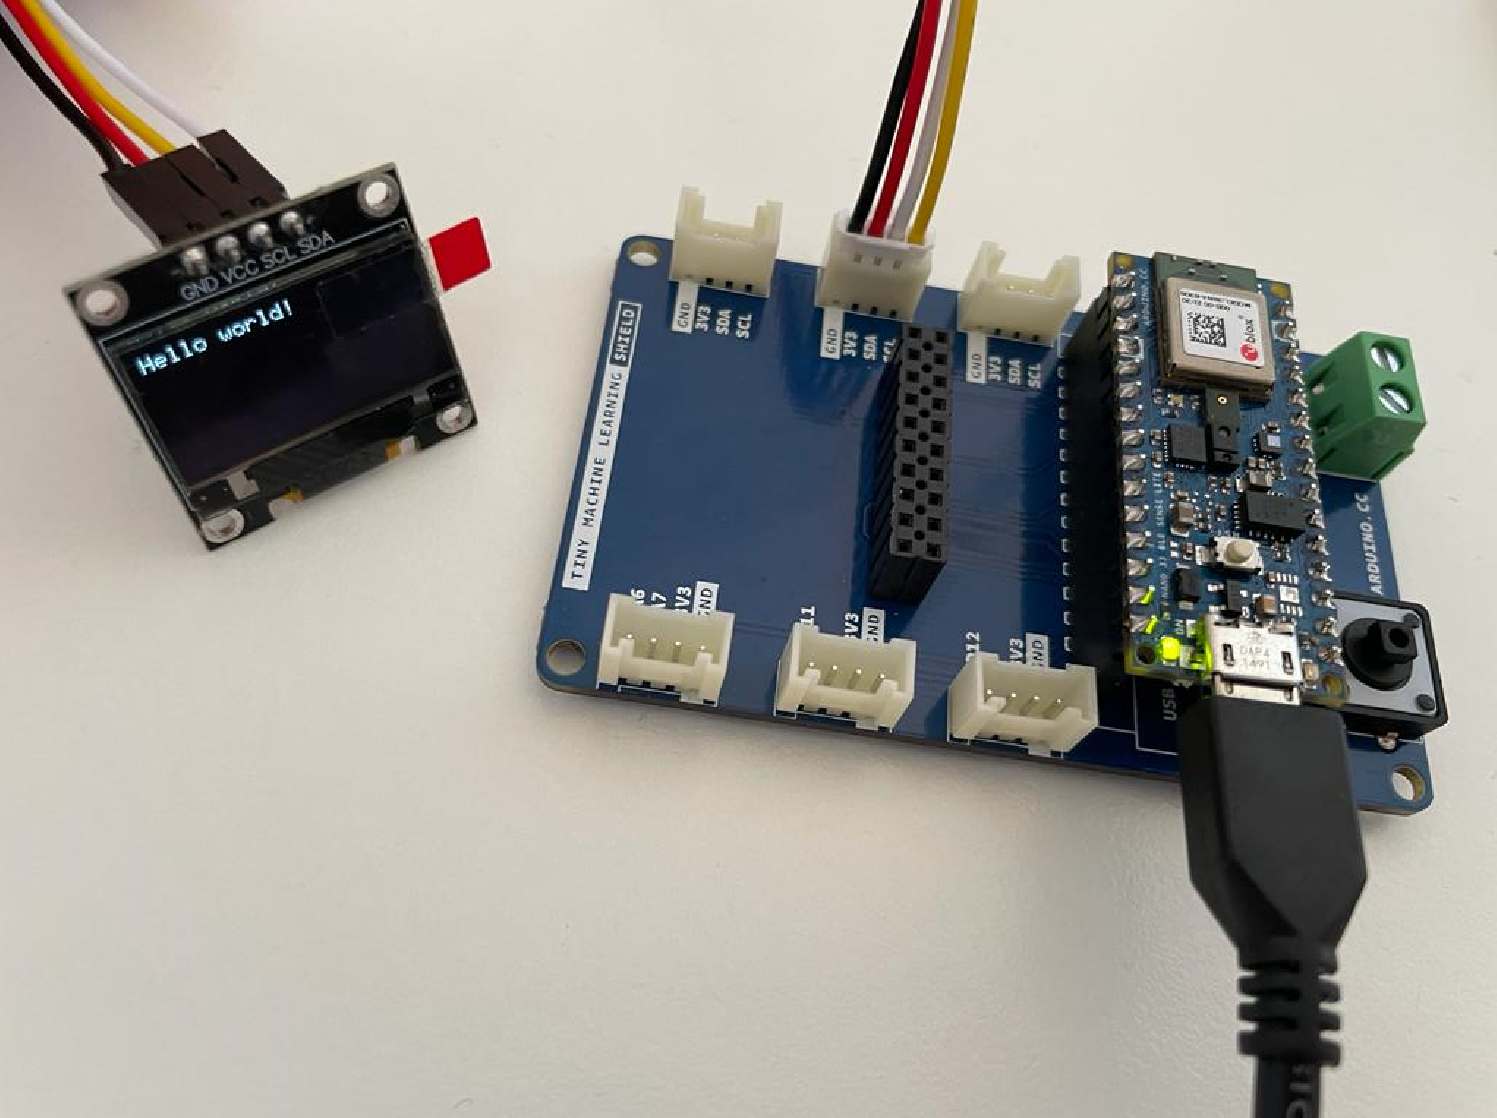
\includegraphics[width=0.9\textwidth]{OLED/OLEDTest}
    \caption{Testausgabe des OLED Display}
\end{figure}

\section{Software}

\subsection{Verwendete Bibliotheken}

Zur Ansteuerung des Displays werden folgende Bibliotheken verwendet:

\begin{itemize}
    \item \FILE{Wire.h}: Diese Bibliothek ermöglicht die Kommunikation über den I2C-Bus, der für die Ansteuerung des OLED-Displays verwendet wird \cite{ArduinoWire:2022}
    \item \FILE{Adafruit-GFX.h}: Eine Grafikbibliothek, die von Adafruit entwickelt wurde und grundlegende Funktionen zur Darstellung von Text und Grafiken auf Displays bietet \cite{AdafruitGFX:2023} 
    \item \FILE{Adafruit-SSD1306.h}: Eine Bibliothek für das  OLED-Display SSD1306, die auf der Adafruit-GFX-Bibliothek basiert\cite{ArduinoSSD:2023} \Mynote{Ist dies kompatibel? Was ist damit möglich?}
\end{itemize}

\subsection{OLED-Display}

Ein Objekt der Klasse \PYTHON{Adafruit\_SSD1306} wird erstellt, um das OLED-Display zu steuern:

\medskip

\PYTHON{Adafruit\_SSD1306 display(SCREEN\_WIDTH, SCREEN\_HEIGHT, \&Wire, -1);}

\medskip

Das Display wird mit der Auflösung 128 Pixel $\times$ 64 Pixel initialisiert:

\medskip

\PYTHON{\#define SCREEN\_WIDTH 128}

\PYTHON{\#define SCREEN\_HEIGHT 64}


\subsection{Initialisierung und Setup}
In der setup()-Methode werden die erforderlichen Initialisierungen durchgeführt:

\begin{itemize}
    \item \PYTHON{display.begin(...)}: Initialisiert das OLED-Display
    \item \PYTHON{display.clearDisplay()}: Löscht den Displayinhalt
    \item \PYTHON{display.setTextColor(WHITE)}: Setzt die Textfarbe auf Weiß
    \item \PYTHON{display.setTextSize(2)}: Setzt die Textgröße auf 2
    \item \PYTHON{pinMode(buttonPin, INPUT\_PULLUP)}: Konfiguriert den Taster-Pin als Eingang mit Pull-Up-Widerstand
    \item \PYTHON{Serial.begin(9600)}: Initialisiert die serielle Kommunikation mit einer Baudrate von 9600
    \item \PYTHON{PDM.onReceive(onPDMdata)}: Registriert den Empfang des Mikrofonsignals als PDM-Signal
\end{itemize} 

\subsection{Messungssteuerung}
Die Funktion \PYTHON{onPDMdata()} wird aufgerufen, wenn Daten vom Mikrofon verfügbar sind. Dies liest die Daten in einen Array ein und zählt die Anzahl der gelesenen Samples:

\begin{figure}[h]
    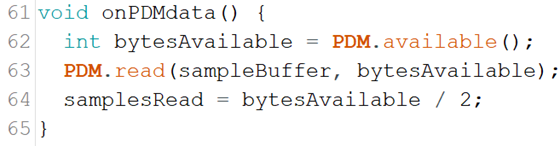
\includegraphics[width=10cm]{OLED/OLEDCode1.png}
    \caption{Code Einlesen/Zählen}
\end{figure}



Die Hauptfunktion \PYTHON{loop()} enthält zwei Funktionen für die Messungssteuerung und die Benutzeroberfläche:

\begin{figure}[h]
    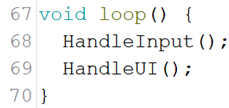
\includegraphics[width=4cm]{OLED/OLEDCode2.png}
    \caption{Code Messungssteuerung}
\end{figure}


Die Funktion \PYTHON{HandleInput()} überwacht den Zustand der beiden Taster und steuert somit den Messungsablauf:

{
    \captionof{code}{Monitoring}\label{Code:OLED:Monitoring}
    \ArduinoExternal{firstline=78,lastline=127}{../../Code/Arduino/OLED/DEBO - OLED2 0.96/TestDeboOLED.ino}
}


\begin{itemize}
    \item Zunächst wird der Zustand der beiden Taster überprüft und die Abfrage nach einem gedrückten Button ist aktiv (\PYTHON{blueButtonIsPressed}, \PYTHON{redButtonIsPressed}).
    \item Wenn der blaue Taster gedrückt wird, wird die Messung gestartet, indem \PYTHON{isMeasuring} auf \PYTHON{true} gesetzt wird und die Funktion \PYTHON{StartSampling()} aufgerufen wird.
    \item Wenn der rote Taster gedrückt wird, wird die Messung beendet, indem \PYTHON{isMeasuring} auf \PYTHON{false} gesetzt wird und die Funktion \PYTHON{StopSampling()} aufgerufen wird. Je nach vorherigem Zustand des roten Tasters wird entweder der maximale Wert SPL in dB angezeigt (\PYTHON{ShowMaxdBspl()}) oder der durchschnittliche dB SPL-Wert (\PYTHON{ShowAveragedBspl()}).
    \item \PYTHON{isDelayOver} wird auf \PYTHON{true} gesetzt, wenn die Startverzögerung (definiert durch \PYTHON{measureThresholdMilliseconds}) von 1200ms abgelaufen ist.
    \item Es gibt eine kurze Verzögerung (\PYTHON{delay(50)}) zwischen den Schleifendurchläufen, um Tastenprellungen zu vermeiden.
\end{itemize} 

\subsection{Mikrofondatenverarbeitung}
Die Funktion \PYTHON{StartSampling()} initialisiert die Datenverarbeitung:

{
    \captionof{code}{Start and stop sampling}\label{Code:Mirco:StartSampling}
    \ArduinoExternal{firstline=129,lastline=138}{../../Code/Arduino/OLED/DEBO - OLED2 0.96/TestDeboOLED.ino}
}

\PYTHON{PDM.begin(1, 16000)}: Initialisiert eine Abtastrate von 16.000 Hz.
Die Funktion \PYTHON{StopSampling()} beendet die Aufnahme von Audiodaten.


\subsection{Anzeige der Ergebnisse}
Die Funktionen \PYTHON{ShowResult()} und \PYTHON{ShowMicrophoneValues()} sind für die Anzeige der Messergebnisse auf dem OLED-Display verantwortlich. \PYTHON{ShowResult()} zeigt den aktuellen SPL-Wert in dB auf dem Display an und aktualisiert den maximalen Wert SPL in dB, wenn nach der Startverzögerung ein neuer Höchstwert erreicht wird. \PYTHON{ShowMicrophoneValues()} verarbeitet die vom Mikrofon empfangenen Signale. Der maximale Samplewert wird ermittelt und verwendet, um den Wert SPL in dB zu berechnen. Die Funktion berechnet auch einen Durchschnittswert über eine bestimmte Zeit, \PYTHON{averagingTime = 200ms}, und zeigt das Ergebnis auf dem Display an. Die Funktionen \PYTHON{ShowMaxdBspl()} und \PYTHON{ShowAveragedBspl()} zeigen den maximalen bzw. den durchschnittlichen Wert SPL in dB auf dem Display an.

\subsection{Umrechnung auf den Wert dBSPL}

Die Umrechnung des Mikrofonsignals auf den dBSPL-Wert erfolgt in der Funktion \PYTHON{getDbValueFromPMC()}:

{
    \captionof{code}{Conversion of the microphone signal} \label{Code:Mirco:StartSampling}
    \ArduinoExternal{firstline=159,lastline=163}{../../Code/Arduino/OLED/DEBO - OLED2 0.96/TestDeboOLED.ino}
}


\PYTHON{MaxSampleVoltage} wird berechnet, indem der maximale Samplewert \PYTHON{maxSampleValue} mit der Referenzspannung des Mikrocontrollers („Vref = 3,3 V“) multipliziert und durch den maximalen Wert eines 16-Bit-Signed-Integers (32767) dividiert wird. 32767 ist der maximale Wert eines 16-Bit-Signed-Integers, der der maximalen Amplitude des Audiosignals entspricht.
Der dB SPL-Wert („dBspl“) wird mit der Formel „20 * log10(Voltage / Vrms) + sensitivity“ berechnet [Quelle der Fomel: PDF Decibels Formula https://physicscourses.colorado.edu/phys3330/phys3330\_sp19/resources/Decibels\_Phys\_3330.pdf University of Colorado System], wobei „Voltage“ der berechnete „maxSampleVoltage“ ist, und „sensitivity“ die Empfindlichkeit des Mikrofons in dBV (Dezibel-Volt) ist. „Vrms“ ist die RMS-Spannung (Root Mean Square), die einem Schalldruckpegel von 94 dB SPL entspricht. Dieser Wert wurde experimentell ermittelt.



\subsection{Benutzeroberfläche}
Die Funktion \PYTHON{HandleUI()} aktualisiert OLED-Display Anzeige:

{
    \captionof{code}{OLED-Aktualisierung}\label{Code:OLED:Update}
    \ArduinoExternal{firstline=227,lastline=234}{../../Code/Arduino/OLED/DEBO - OLED2 0.96/TestDeboOLED.ino}
}

\begin{figure}[h]
    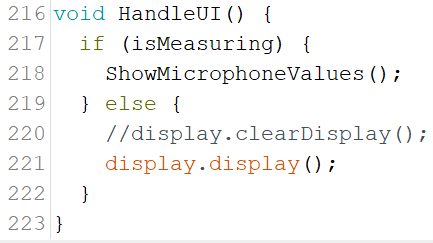
\includegraphics[width=8cm]{OLED/OLEDCode7.png}
    \caption{Code }
\end{figure}

Wenn eine Messung aktiv ist („isMeasuring == true“), werden die aktuellen Messwerte auf dem Display angezeigt. Andernfalls wird der Displayinhalt aktualisiert, ohne neue Werte anzuzeigen.


\section{Das OLED-Display SSD1306}
Das OLED-Display SSD1306 dient dazu, die Messwerte des Arduinos auszugeben. Es besitzt eine Maße von ca. 27 x 27 x 4,1 mm und ist durch seinen hohen Kontrast sehr gut lesbar. Das Display besteht aus 128x64 OLED Bildpunkten, die durch den Chip SSD1306 gesteuert werden können. Das Display benötigt eine Betriebsspannung von 3,3 V bis 5 V und hat einen Stromverbrauch von 0,04 W im normalen Betrieb. Die Betriebstemperatur von -30 °C bis +80 °C sollte dabei nicht überschritten werden. Angesteuert werden kann das Display über die Schnittstelle I2C mit den Pins VCC, GND, SCL und SDA. Mit Hilfe der beiden Bibliotheken Adafruit GFX und Adafruit SSD1306 kann das Display programmiert werden. Hierzu aber mehr in dem Kapitel \label{key}
\begin{figure}[h]
    \centering
    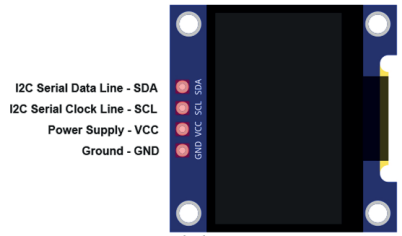
\includegraphics[width=0.5\textwidth] {OLED/OLEDDisplay}
    \caption{Pins des OLED-Displays.}
    \label{fig:OLEDDisplay}
\end{figure}

Das Display verfügt über vier Pins, welche in der Abbildung \ref{fig:OLEDDisplay} zu sehen sind.

Der VCC-Pin, der für die Spannungsversorgung des Geräts sorgt, wird mit dem 5V-Pin des Mikrocontrollers verbunden. Der GND-Pin des Geräts wird mit dem GND-Pin des Mikrokontrollers verbunden, um eine gemeinsame Masseverbindung herzustellen. Der SDA-Pin des Geräts muss entweder mit dem speziellen SDA-Pin oberhalb des Pin 13 oder mit dem analogen Pin A4 des Mikrocontrollers verbunden werden. Der SCL-Pin des Geräts wird entweder mit dem speziellen SCL-Pin oberhalb des Pin 13 oder alternativ mit dem analogen Pin A5 des Mikrocontrollers verbunden. \cite{AZ-Delivery:2023,FunduinoOLED:2023}

\section{Schaltplan des Aufbaus}
Der folgende Schaltplan stellt die Komponenten des Arduino Nano BLE Sense Lite, des Sensors BME280 und des OLED-Displays dar. Als Spannungsquelle dient ein Computer, der den Arduino Nano 33 BLE Sense über ein USB-A auf Mikro-USB Kabel versorgt. Die Komponenten sind sinngemäß miteinander verbunden und in Abbildung \ref{fig:Schaltplan} abgebildet.

\begin{figure}[h]
    \centering
    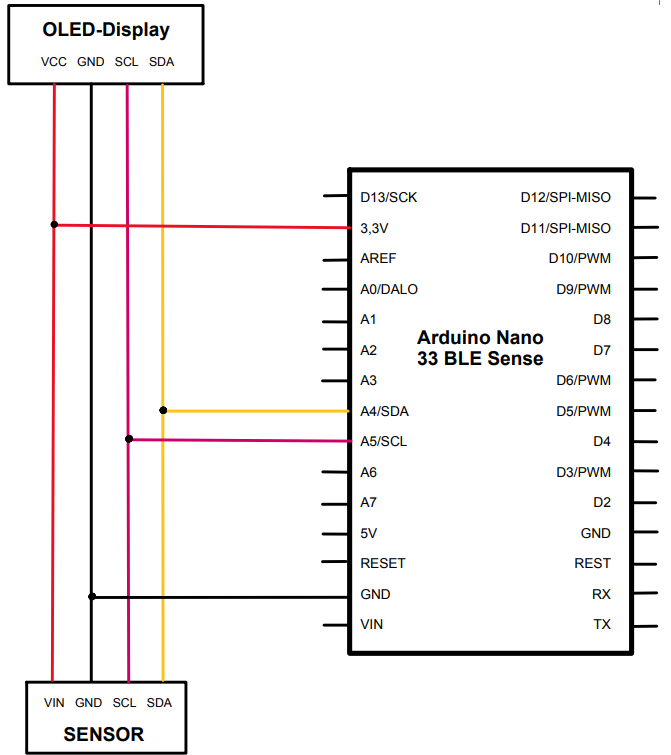
\includegraphics[width=0.5\textwidth] {OLED/OLEDCircuit3}
    \caption{Stationärer Aufbau der Wetterstation}
    \label{fig:Schaltplan} \cite{ArduinoNano33Manual:2022}
\end{figure}

\section{Genutzte Bibliotheken}
Bei Bibliotheken handelt es sich um Ansammlungen von dem Code und Funktionen für bestimmte Anwendungen oder Hardware. Diese werden oft genutzt um Aufgaben leichter lösen zu können und ein neu schreiben von komplexen Funktionen zu vermeiden. In unserem Fall verwenden wir Bibliotheken für den Arduino, den Sensor BME280 und das OLED-Display.

\subsection{Bibliothek Wire.h}
Die Bibliothek Wire.h ist eine Standardbibliothek für Arduino-Plattformen, welche Funktionen und Methoden für die Kommunikation zur Verfügung stellt. Mit Hilfe der Schnittstelle I2C ermöglicht die Bibliothek die Kommunikation zwischen einem Arduino und einem anderen I2C-fähigen Gerät wie z.B. Sensoren oder Displays. I2C ist ein Kommunikationsbus, der im Vergleich zu seriellen Schnittstellen den Vorteil hat, dass er mit mehr als zwei Geräten kommunizieren kann. Ein I2C-Bus benötigt zwei Leitungen: SCL für ein Taktsignal und SDA für Daten.
Um die Wire.h Bibliotek anwenden zu können, muss sie am Anfang des Sketchs eingebunden werden: \textit{\#include<….h>} \cite{W3CWire:2023}


\subsection{Bibliothek SSD1306Ascii.h für das Testprogramm}
Bei der Bibliothek SSD1306Ascii.h handelt es sich um eine benutzerdefinierte Bibliothek, die ähnlich zu der Adafruit Bibliothek SSD1306 ist. Beide sind für die Ansteuerung von OLED-Displays notwendig und basieren auf den Controller-Chip SSD1306. Sie ermöglichen das einfache Schreiben von den Text, Zeichen von Formen und Anzeigen von Bitmap-Bildern auf dem Display. 
Um die Bibliothek SSD1306Ascii.h zu verwenden, muss sie erst als ZIP-Datei heruntergeladen und anschließend von dem Arduino Library Manager installiert werden. Mit Hilfe von \textit{\#include<SSD1306Ascii.h>} kann man sie in dem Arduino-Code einbinden. \cite{FunduinoBME280:2023}


\subsection{Testen des OLED-Displays }
Für die Programmierung des Displays gibt es viele Möglichkeiten. Da es viele Librarys gibt, muss zuerst einmal überlegt werden, welche verwendet werden sollen. Um einen ersten Eindruck über die Programmierung des Displays zu bekommen, wurde zunächst ein Beispielsketch getestet. Es handelt sich hier um den Sketch \FILE{Hello World}, welcher unter Datei -> SSD1206Ascii -> HelloWorldWire zu finden ist (siehe Abbildung\ref{fig:TestprogrammDisplay}).

\begin{figure}
    \centering
    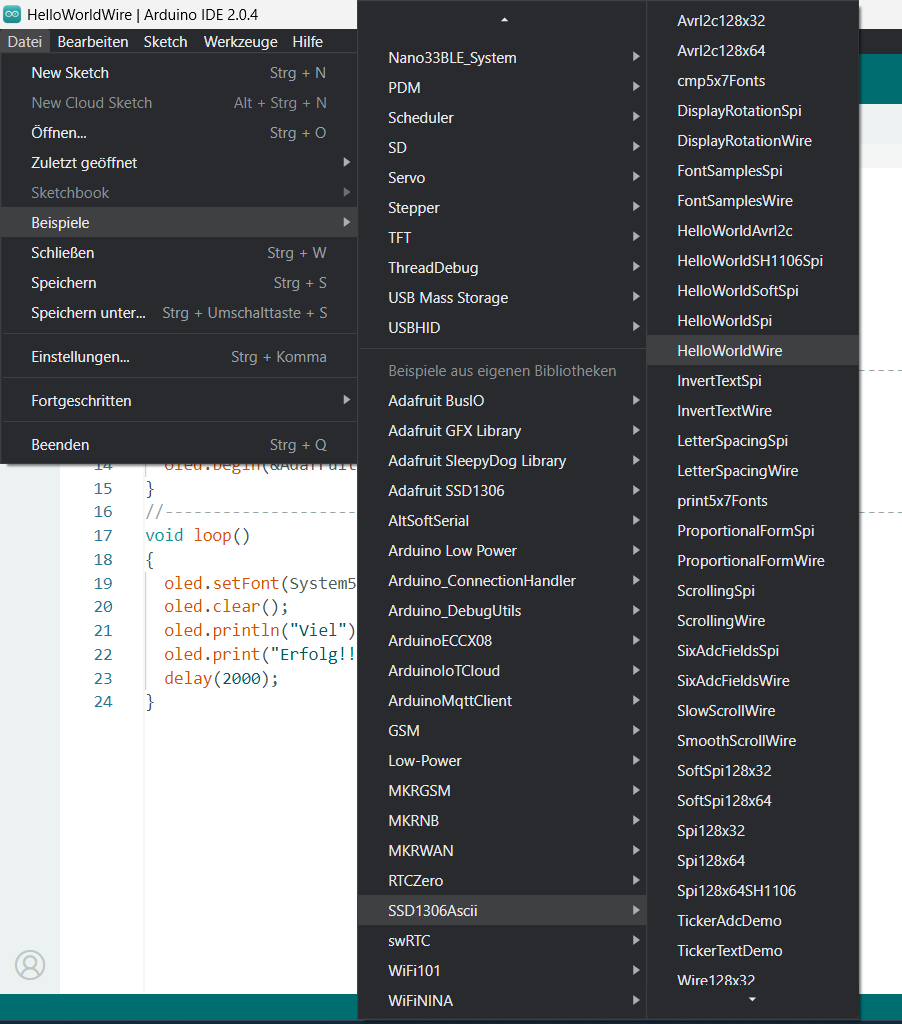
\includegraphics[width=1\textwidth] {OLED/TestprogrammDisplay}
    \captionof{figure}{Pfad des Testprogramms.}
    \label{fig:TestprogrammDisplay}
\end{figure}

Das Testprogramm \FILE{Hello World} (siehe Seite \pageref{Test1}) wird dafür benutzt, um den Text Hello World auf dem Display auszugeben (siehe Abbildung \ref{fig:ErsteAusgabeDisplay}). Es wird hier verwendet, um sich mit der Software vertraut zu machen und um sicherzustellen, dass die Entwicklungsumgebung richtig eingerichtet ist. Außerdem wird getestet, ob das Programmieren funktioniert und alle Kabel richtig angesteckt sind.

\bigskip

{
    \captionof{code}{Simple program for OLED displays}\label{Code:OLED:Sample}
    \ArduinoExternal{firstline=227,lastline=234}{../../Code/Arduino/OLED/Grove - OLED Display SSD1308/TestSSD1306.ino}\label{Test1}
}


Nachdem der Quellcode kompiliert und an den Arduino geschickt wurde, wurde auf dem Display der Text Viel Erfolg ausgegeben (siehe Abbildung \ref{fig:ErsteAusgabeDisplay}). Hiermit ist sichergestellt worden, dass die Entwicklungsumgebung und der Compiler korrekt funktionieren. \cite{FunduinoBME280:2023}

\begin{figure}
    \centering
    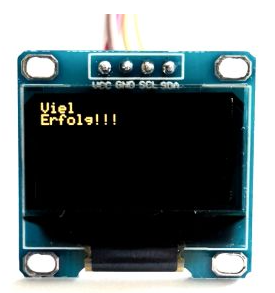
\includegraphics[width=0.5\textwidth] {OLED/Output}
    \captionof{figure}{Erste Ausgabe Display} 
    \label{fig:ErsteAusgabeDisplay} \cite{FunduinoOLED:2023}
\end{figure}


\section{Beispiel eines  OLED-Displays}

Zur Ausgabe unserer Messwerte verwenden wir ein 0,96 Zoll OLED Display, welches über den I\textsuperscript{2}C Port mit dem Tiny Machine Learning Shield verbunden ist. Es verfügt über die Anschlüsse SDA und SCL zur Datenübertragung, über VCC zur Spannungsversorgung und GND für die Masse. Außerdem ist es mit einem internen Spannungsregler ausgestattet, der 3,3V- und 5V-Betrieb ermöglicht.

\begin{figure}[H]
    \centering
    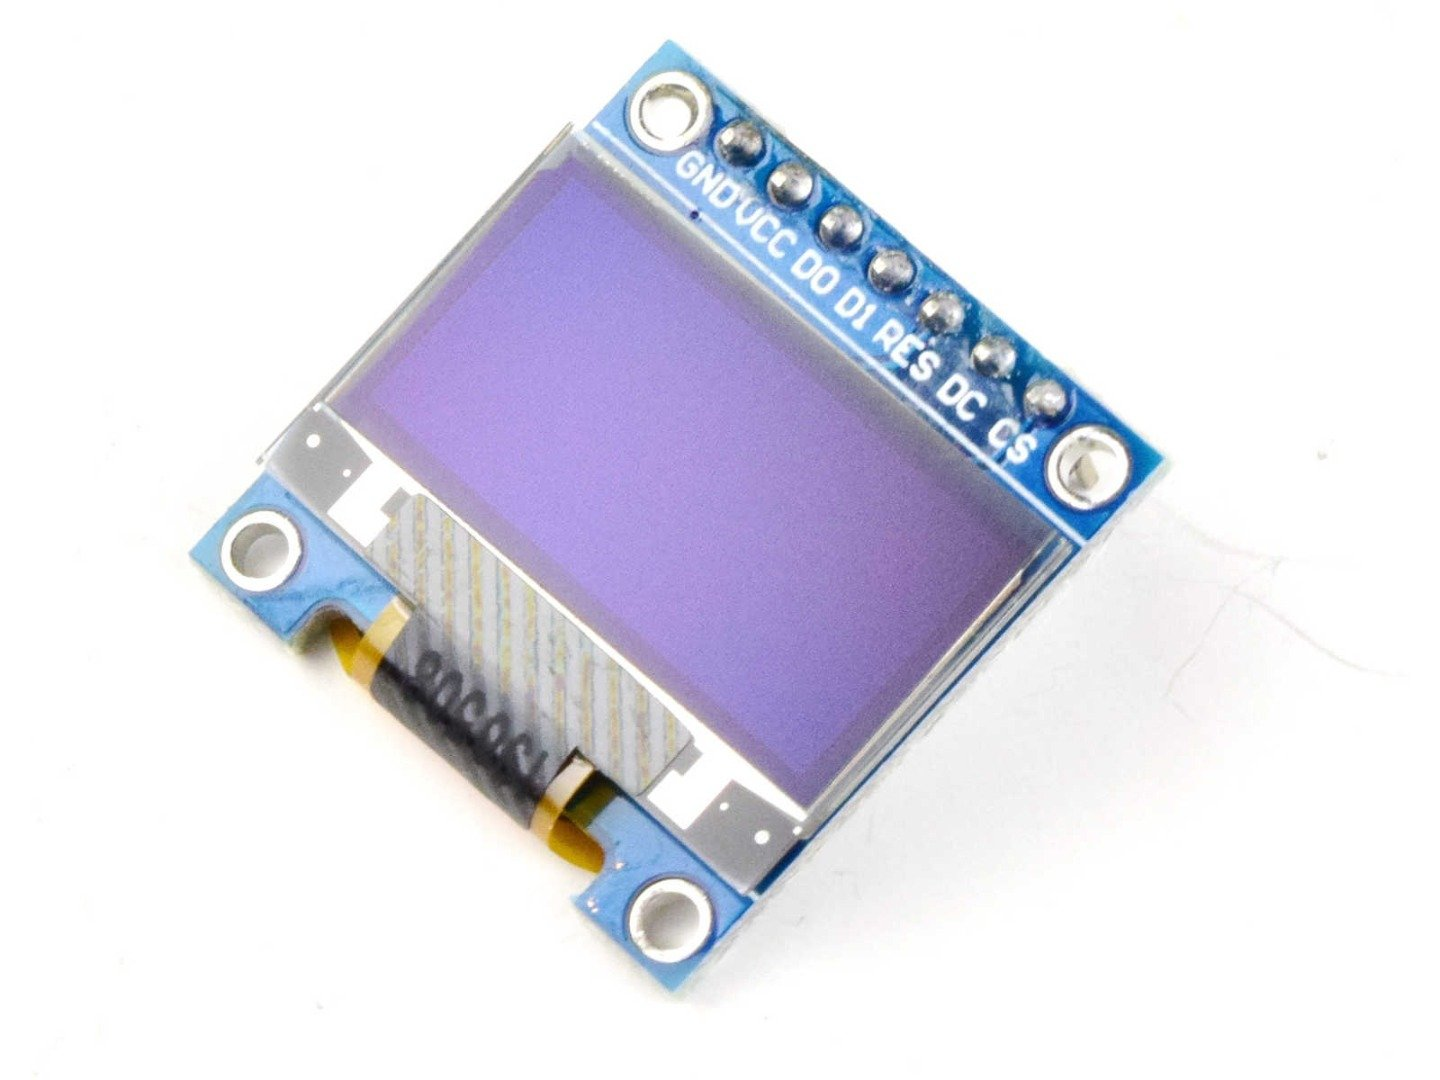
\includegraphics[width=0.8\textwidth]{Nano33BLESense/TinyMLKit/display.jpg}
    \caption{Das Display zur Ausgabe der Messwerte}
\end{figure}
\Mynote{Quelle fehlt, Infos, \ldots}

Quelle: \HREF{https://www.reichelt.de/arduino-display-0-96-grove-oled-display-ssd1308-grv-oled-0-96-p191252.html}{Arduino - Display 0,96'', Grove OLED-Display, SSD}


\bigskip

Allgemeines

\begin{tabular}{ll}
Typ  & OLED \\
Ausführung &  Zubehör \\
Farbe  & monochrom \\
\end{tabular}
Display

\begin{tabular}{ll}
Display  & bis 1,9 Zoll \\
Diagonale  & 1,0 Zoll \\
Auflösung, physik. &  128 x 64 Pixel \\
Diagonale  & 2,44 cm \\
\end{tabular}

Ausführung
\begin{tabular}{ll}
Modell  & Arduino \\
\end{tabular}
Besonderheiten

\begin{tabular}{ll}
Besonderheit  & - \\
\end{tabular}

Sonstiges
\begin{tabular}{ll}
Spezifikation &  SSD1308 \\
\end{tabular}

Herstellerangaben

\begin{tabular}{ll}
Hersteller &  SEEED \\
Artikelnummer des Herstellers &  104030008 \\
Verpackungsgewicht  & 0.01 kg \\
\end{tabular}



\subsection{OLED}


Als weiteren Punkt werden Klassenobjekte im Header initialisiert und Adressen von Peripheriegeräten festgelegt. In diesem Fall sind es das Objekt \textit{oled} der Klasse \textit{SSD1306AsciiWire} und die Definition der Adresse des OLED-Displays. Die Adresse wurde zuvor durch einen I$^2$-Scanner bestätigt.

\begin{Arduino}		
    #define I2C_ADDRESS 0x3C  
    SSD1306AsciiWire oled;  
\end{Arduino}

Ein weiterer Punkt ist die Initialisierung und Deklarierung von globalen Variablen. Beim Farberkennungsautomaten sind es zwei Variablen. Über Pin D11, kurz 11, wird der Messtaster abgefragt. Pin D12, kurz 12, gibt bei Bedarf ein Signal an die externe RGB-LED. Durch das Voranstellen von \textit{const} werden beide Variablen zu Konstanten und könne außer über den Source-Code nicht geändert werden. Dies ergibt Sinn, da die Verkabelung sich nicht verändern wird und somit auch nicht die gewählten Pins.

\begin{Arduino}		
    const int TasterPin = 11; 
    const int LedPin = 12;   
\end{Arduino}

\subsubsection{\PYTHON{void setup}\{\}}

In der \textit{setup()}-Funktion wird zuerst die serielle Kommunikation mit einer Baudrate von 9600 bit/s gestartet. Baudrate oder auch Bitrate beschreibt die Übertragungsdauer eines Bits. Bei einer Baudrate von 9600 dauert es 104,17 \textmu s um ein Bit zu übertragen. Je höher die Baudrate ist, desto schneller wird ein Bit übertragen. Der Empfänger tastet meist mehrmals pro gesendetem Bit ab und bildet dann nach dreimaligem Abtasten den Mittelwert, welcher dann als empfangenes Bit weiterverarbeitet wird \cite{Gehrke:2022}.Nach dem Starten der seriellen Kommunikation werden die Modi der zwei genutzten Pins definiert. 

\begin{Arduino}		
    Serial.begin(9600);
    pinMode(buttonPin, INPUT);
    pinMode(ledPin, OUTPUT);
\end{Arduino}

Manche Pins können als Input oder als Output genutzt werden. Im Fall des Arduino Nano 33 BLE Sense Lite sind die Pins D13, AREF, A0-A7, TX, RX und D2-D12 als \ac{gpio} nutzbar. Über das genutzte Shield kann auf A6, A7, D11 und D12 zugegriffen werden. Genutzt werden D11 und D12. Der Tasterpin D11 wird als Input definiert um das Signal aufnehmen zu können, welches durch Drücken des Tasters ausgelöst wird. Pin D12 wird als Output definiert um die externe \ac{rgb}-\ac{led} einzuschalten. Der Befehl \textit{pinMode()} beinhaltet zusätzlich noch die Möglichkeit einen internen Pull-Up-Widerstand einzuschalten \cite{ArduinoPinMode:2019}. 



Anschließend wird das I$^2$C-Protokoll mit dem Objekt \textit{Wire} und der Funktion \textit{begin()} gestartet. Dabei wird der Arduino als Master im I$^2$C-Protokoll angemeldet\cite{ArduinoWire:2022}. Anschließend wird die Taktfrequenz mit 400kHz festgelegt \cite{ArduinoWireClock:2022}.

\begin{lstlisting}		
    Wire.begin();
    Wire.setClock(400000L);
\end{lstlisting}

Im nächsten Schritt wird das OLED-Display gestartet. Hierfür wird mit dem Objekt \textit{oled} die Funktion \textit{begin()} aufgerufen. Dieser Befehl benötigt als Funktionsparameter eine Geräteinitialisierung und die Adresse des Displays. Für die Initialisierungsphase des Farberkennungsautomaten wird ein der Text \textit{INITIALISIERUNG!} auf dem Display ausgegeben. Hierfür wird die Schriftart und die Startposition des Textes auf dem Display festgelegt \cite{ArduinoSSD:2023}.

\begin{lstlisting}		
    oled.begin(&Adafruit128x64, I2C_ADDRESS);
    oled.setFont(System5x7);
    oled.setCursor(0, 40);
    oled.println("INITIALISIERUNG!\n");
\end{lstlisting}
Der letzte Schritt in der \textit{setup()}-Funktion ist das dreimalige Blinken der externen RGB-LED. Hierfür wird eine for-Schleife genutzt. Innerhalb dieser Schleife wird die LED nach 2 s für 0,2 ms eingeschaltet und danach wieder ausgeschaltet. Anschließend wird der Bildschirm gelöscht.

\begin{lstlisting}
    for (int zaehler = 1; zaehler < 4; zaehler = zaehler + 1) {
        delay(2000);
        digitalWrite(LedPin, HIGH);
        delay(200);
        digitalWrite(LedPin, LOW);
        delay(200);
    }
    oled.clear();
\end{lstlisting}


